\begin{Figure}
    \HEADING{1. Why Multiscale?}

        \TEXT{Memory and plasticity involve brain mechanisms from molecular scale to
                enormous networks.}


        \begin{tikzpicture}[
        image/.style = {xslant=0.0,yslant=0.0}
        ]
        \LARGE
        \def\lengthScaleFactor{1.4}
        \def\timeScaleFactor{1.5}

        \newcommand\scaleNode[1]{
            (0, #1*\timeScaleFactor)
        }

        \coordinate (sizeRoot) at (0, 1);
        \coordinate (sizeends) at (0,-1+10*\lengthScaleFactor);
        \coordinate (timeRoot) at (1,0);
        \coordinate (timeends) at (1+11*\timeScaleFactor, 0);


        \draw[-fast cap, yellow!100, line width=4ex]  (timeRoot) to[] (timeends);
        \draw[-fast cap, yellow!100, line width=4ex]  (sizeRoot) to[] (sizeends);


        \node[] (nm) at (0,1) {$nm$};
        \node[] (um) at (0,3.5) {$\mu m$};
        \node[] (mm) at (0,7) {$mm$};
        \node[] (m) at (0,10.5) {$m$};

        \node[] (us) at (1.5,0) {$\mu$ sec};
        \node[] (ms) at (4.0,0) {$m$ sec};
        \node[] (s) at (6.5,0) {sec};
        \node[] (hrs) at (8.5, 0) {hours};
        \node[] (days) at (11.5, 0) {days};

        %% Distance between images and y-axis.
        \def\shifty{-3.0cm}

        \node[image] (n1) at ([xshift=\shifty,yshift=0cm]nm) {
            \includegraphics[width=0.1\textwidth]{images/8tim_TIM_barrel.png}
        };

        \node[image] (n2) at ([xshift=\shifty,yshift=0cm]um) {
            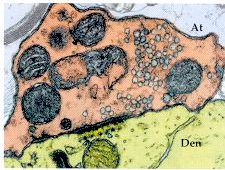
\includegraphics[width=0.1\textwidth]{images/dendrite.png}
        };

        \node[image] (n3) at ([xshift=\shifty,yshift=-1cm]mm) {
            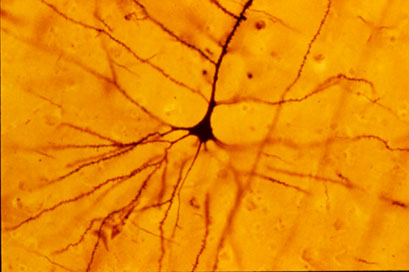
\includegraphics[width=0.1\textwidth]{images/GolgiStainedPyramidalCell.jpg}
        };

        \node[image] (n5) at ([xshift=\shifty,yshift=-1.0cm]m) {
            \includegraphics[width=0.1\textwidth]{images/brain.png}
        };

        \node[image] (n4) at ([xshift=\shifty,yshift=1cm]mm) {
            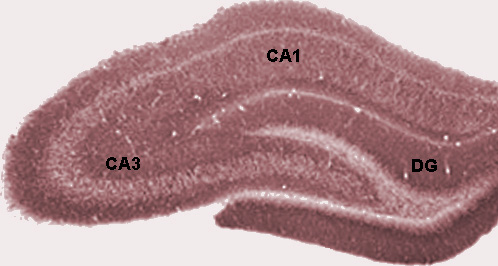
\includegraphics[width=0.1\textwidth]{images/HippocampalRegions.jpg}
        };


        \node[rectangle, minimum width=12cm, minimum height=6.0cm,
        rounded corners, opacity=0.3, fill=blue!50] (chemical) at (10.0,4.5) {};

        \node[] (caption) at ([yshift=-1cm]chemical.north) {\LARGE CHEMICAL};

        \node[rectangle, minimum width=4.5cm, minimum height=5cm
        , opacity=0.5, fill=green!50, rounded corners
            ] (electrical) at (3.8, 8.5) {};

        \node[] at (electrical.center) {\LARGE ELECTRICAL};


        % Put chemical network here
        \node[] (network) at (7.0,4.0) {
            \includegraphics[width=5cm]{images/chemical_reactions.png}
        };

        \node[] (chromosome) at (12.0,5) {
            
\includegraphics[width=5cm]{images/chromosome.png}
        };

        \node[] (text) at ([xshift=5.5cm,yshift=2cm]electrical.east) {
            \begin{minipage}{0.35\textwidth}
                \begin{itemize}[label={}]
                    \item \LARGE{$10^{11}$ cells, $10^{15}$ synapses, $\sim 10000$
                            reactions per synapse}
                    \item \LARGE{Electrical events: $\sim 1$ ms,  Chemical events: $1\;
                        \text{sec} \rightarrow 1000\; \text{sec}$}
                    \item \LARGE{Structural events: $100\; \text{sec}
                        \rightarrow \text{months}$}
                \end{itemize}
            \end{minipage}
        };

    \end{tikzpicture} %
    \begin{tikzpicture}
        \def\figwidth{0.1\textwidth}
        \def\captionwidth{0.28\textwidth}
        \node[] (stochastic) {
            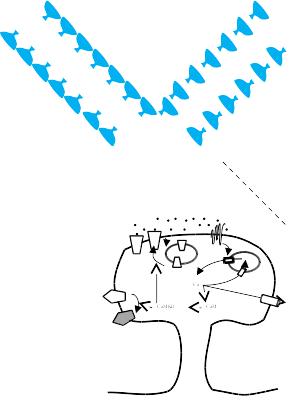
\includegraphics[height=\figwidth]{./images/stochastic_solver.png}
        }; 
        \node[text width=\captionwidth] at ([yshift=-0.5cm]stochastic.south)
        {\LARGE{\bf Reaction at single molecule level}
        };
        \node[] (ksolve) at ([yshift=-3cm]stochastic.south) {
            \includegraphics[height=\figwidth]{./images/ksolve_dsolve.png}
        };
        \node[text width=\captionwidth] at ([yshift=-0.0cm]ksolve.south) {
            \LARGE{\bf Reaction Diffusion Solver}};
        \node[] (hsolve) at ([yshift=-3cm]ksolve.south) {
            \includegraphics[height=\figwidth]{./images/hsolve.png}
        };
        \node[text width=\captionwidth] at ([yshift=-0.0cm]hsolve.south) {
            \LARGE{\bf Electrical: Hines Solver}};
    \end{tikzpicture}

    \vspace{2cm}
    \TEXT{We have developed \textcolor{black}{\textsc{MOOSE}}: Multiscale
            Object Oriented Simulation Environment, to model plasticity and brain
            computation across scales.}

    %% Here goes MOOSE picture.

    \vspace{2cm}

    \SECTION{2.1 Modelling Memory}

     \begin{tikzpicture}[
        spy using outlines={circle
            , magnification=10, connect spies
        }
                 ]
         \centering
         \node [] (image) at (0,-1) {
             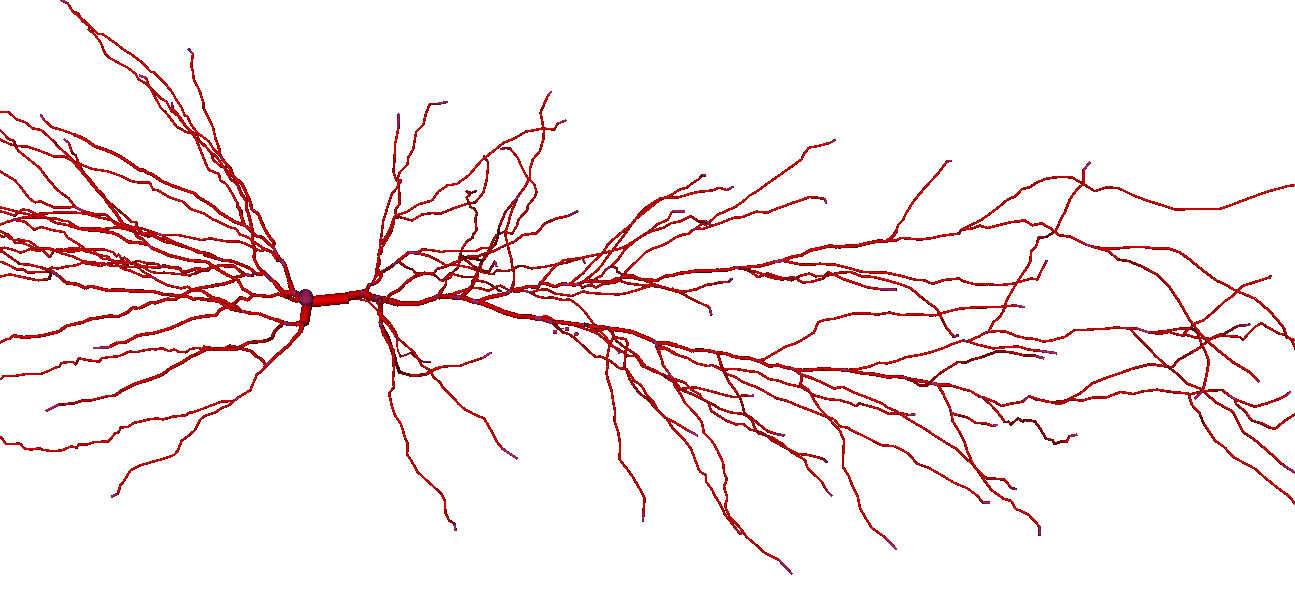
\includegraphics[scale=0.2,angle=-30]{./images/ca1_neuron.png}
         };

         \foreach \i in {-3,...,3}
         \foreach \j in {-3,...,3}
         {
             \node[fill=blue,opacity=0.3,thin,inner sep=0pt, minimum size=3mm,circle] (n\i\j) at (\i, \j) {};
         };

         \spy[blue, size=3cm] on (1.65, -1.5) in node[left] at (7,3);
         \node[below=4cm,text width=0.3\textwidth] {\CAPTION{A single detailed neuron is
                 embedded in a network of simple cells}};

         %% Cool. Now create a 3d compartment model here.
         \begin{scope}[xshift=11cm, yshift=3cm
             , compartment/.style={cylinder
                 , draw
                 , cylinder uses custom fill
                 , cylinder end fill = red!35
                 , cylinder body fill = red!40
                 , inner sep = 3mm
                 , minimum height = 1cm
                 , minimum width = 1cm 
             }
             , spine/.style={cylinder 
                 , fill = blue!20
                 , inner sep=1mm
                 , minimum height=1mm
                 , minimum width=3mm
             }
             , branch/.style={cylinder
                 , draw
                 , cylinder uses custom fill
                 , cylinder end fill = red!35
                 , cylinder body fill = red!40
                 , minimum height = 1.5cm
                 , minimum width = 0.5cm
                 , inner sep = 1mm
             }
             ]

             \node[compartment] (c1) {};
             \node[compartment] (c2) at (c1.east) {};
             \node[compartment] (c3) at (c2.east) {};

             \node[branch,rotate=45] (b1) at ([xshift=4mm,yshift=2mm]c3.before top) {};
             \node[branch,rotate=-45] (b2) at ([xshift=1mm, yshift=-7mm]c3.base east) {};

             % Spines
             \node[spine, inner sep=1mm, rotate=135] (s11) at (b1.north east) {};
             \node[spine, inner sep=1mm, rotate=135] (s12) at ([xshift=3mm]b1.south east) {};

             \node[spine, inner sep=1mm, rotate=45] (s21) at (b2.north east) {};
             \node[spine, inner sep=1mm, rotate=45] (s22) at ([xshift=-3mm]b2.south east) {};

         \end{scope}

         %% Scope to draw chemisty 
         \begin{scope}

             \node[] (chemical) at ([yshift=-6cm]c2.south) {
                 \includegraphics[width=0.35\textwidth, trim=5mm 5mm 5mm 5mm, clip]{./images/chemical_reactions.png}
             };

             %%  
             \node [above] (chemicallabel) at ([yshift=-2cm]c1.south) {\LARGE{
                     Chemical models}};

             \draw[o-o] (c1.center) to [bend right] (chemicallabel.center);
            
             %% Add transportation model.
             \node[] (transport) at ([xshift=7cm,yshift=-3cm]s12.north) {
                 \includegraphics[width=0.3\textwidth]{./images/transport_mechanism.png}
             };

             \node[] (tlabel) at ([xshift=0.5cm, yshift=0cm]transport.north) {\LARGE{Trafficking
                     models}};

             \draw[o-o] (s21.center) to [bend left] (tlabel) ;

         \end{scope}
     \end{tikzpicture}


     \vspace{1cm}
     \begin{tikzpicture}
         \node[] (label) at ([xshift=-20cm]tlabel) {
             \CAPTION{\hspace{12cm} Neighbouring spines are modified differently}
         };
     \end{tikzpicture}

     %% memory results by upi
    \begin{tikzpicture}
         \node[] (resultb) {
             \includegraphics[width=0.5\textwidth]{./images/spike_raster.png}
         };
     \end{tikzpicture} \hfill %
     \begin{tikzpicture}
         \node[] (resultA) {
             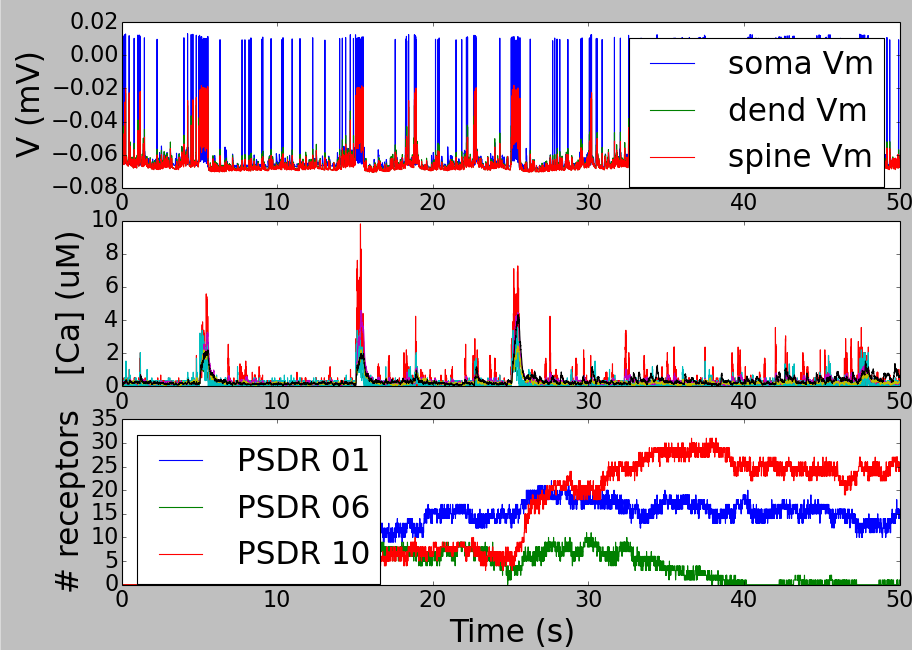
\includegraphics[width=0.5\textwidth]{./images/timeseries.png}
         };
     \end{tikzpicture}
 

\end{Figure}
